\documentclass[tikz]{standalone}
\usetikzlibrary{chains,positioning,trees}
\begin{document}
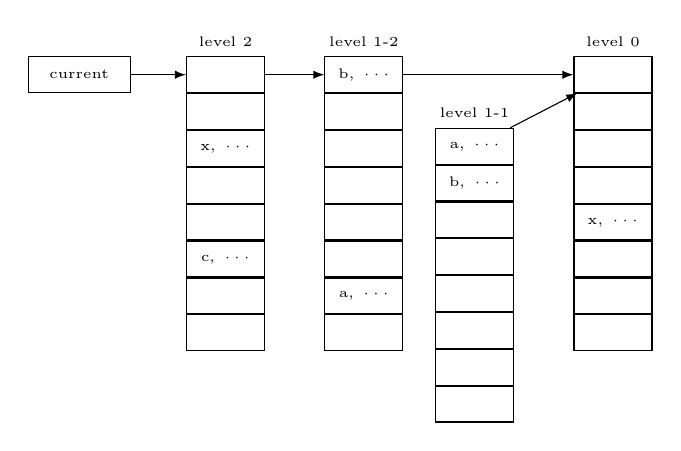
\begin{tikzpicture}[
  node distance = 0ex and 5ex,
  start chain = going below,
  base/.style = {
    rectangle,
    draw,
    fill=#1,
    % inner sep=0mm,
    minimum height=3ex,
    text width=5ex,
    align=center,
    font=\linespread{.9}\selectfont
  },
  box/.style = {base=#1, on chain},
  arr/.style = {thin,-latex},
  ]
  {
    [start chain]
    \coordinate[on chain] (level2);
    \node[box=white] (level2N) {};
    \node[box=white] {};
    \node[box=white] {\tiny x, \(\cdots\)};
    \node[box=white] {};
    \node[box=white] {};
    \node[box=white] {\tiny c, \(\cdots\)};
    \node[box=white] {};
    \node[box=white] {};
  }
  {
    [start chain]
    \coordinate[on chain, right=5em of level2] (level12);
    \node[box=white] (level12N) {\tiny b, \(\cdots\)};
    \node[box=white] {};
    \node[box=white] {};
    \node[box=white] {};
    \node[box=white] {};
    \node[box=white] {};
    \node[box=white] {\tiny a, \(\cdots\)};
    \node[box=white] {};
  }
  {
    [start chain]
    \coordinate[right=4em of level12] (level11v);
    \coordinate[on chain, below=6ex of level11v] (level11);
    \node[box=white] (level11N) {\tiny a, \(\cdots\)};
    \node[box=white] {\tiny b, \(\cdots\)};
    \node[box=white] {};
    \node[box=white] {};
    \node[box=white] {};
    \node[box=white] {};
    \node[box=white] {};
    \node[box=white] {};
  }
  {
    [start chain]
    \coordinate[on chain, right=9em of level12] (level0);
    \node[box=white] (level0N) {};
    \node[box=white] {};
    \node[box=white] {};
    \node[box=white] {};
    \node[box=white] {\tiny x, \(\cdots\)};
    \node[box=white] {};
    \node[box=white] {};
    \node[box=white] {};
  }
  \node[box=white, text width=7ex, left=2em of level2N] (current) {\tiny current};
  \node[rectangle, above=of level2] {\tiny level 2};
  \node[rectangle, above=of level12] {\tiny level 1-2};
  \node[rectangle, above=of level11] {\tiny level 1-1};
  \node[rectangle, above=of level0] {\tiny level 0};
  \draw[arr] (current) -- (level2N);
  \draw[arr] (level2N) -- (level12N);
  \draw[arr] (level12N) -- (level0N);
  \draw[arr] (level11N) -- (level0N);
\end{tikzpicture}
\end{document}
